\section{Áttekintés}

A rendszer működéséhez szükséges egy szerver, ami Wi-Fi vagy XBee alapú rádiós
kommunikáció segítségével fogadja az adatokat a drónoktól, valamint továbbítja
feléjük a kiadott parancsokat. Ehhez a szerver a felhasználói kliens WebSocket
protokoll segítségével csatlakozhat. A kliens program futtatható oly módon, hogy
egy központi webszerver egy helyi hálózaton kiszolgálja a FlockWave kliens
alkalmazás webes tartalmát (csomagolt JavaScript, stíluslapok, képek, stb.), így
ez tetszőleges olyan eszközről elérhető, amely rendelkezik (lehetőség szerint
Google Chrome) böngészővel, illetve Windows, Linux és MacOS (OSX) rendszerekre
elérhető Electron segítségével becsomagolt önműködő állomány is.

\begin{figure}[H]
  \centering
    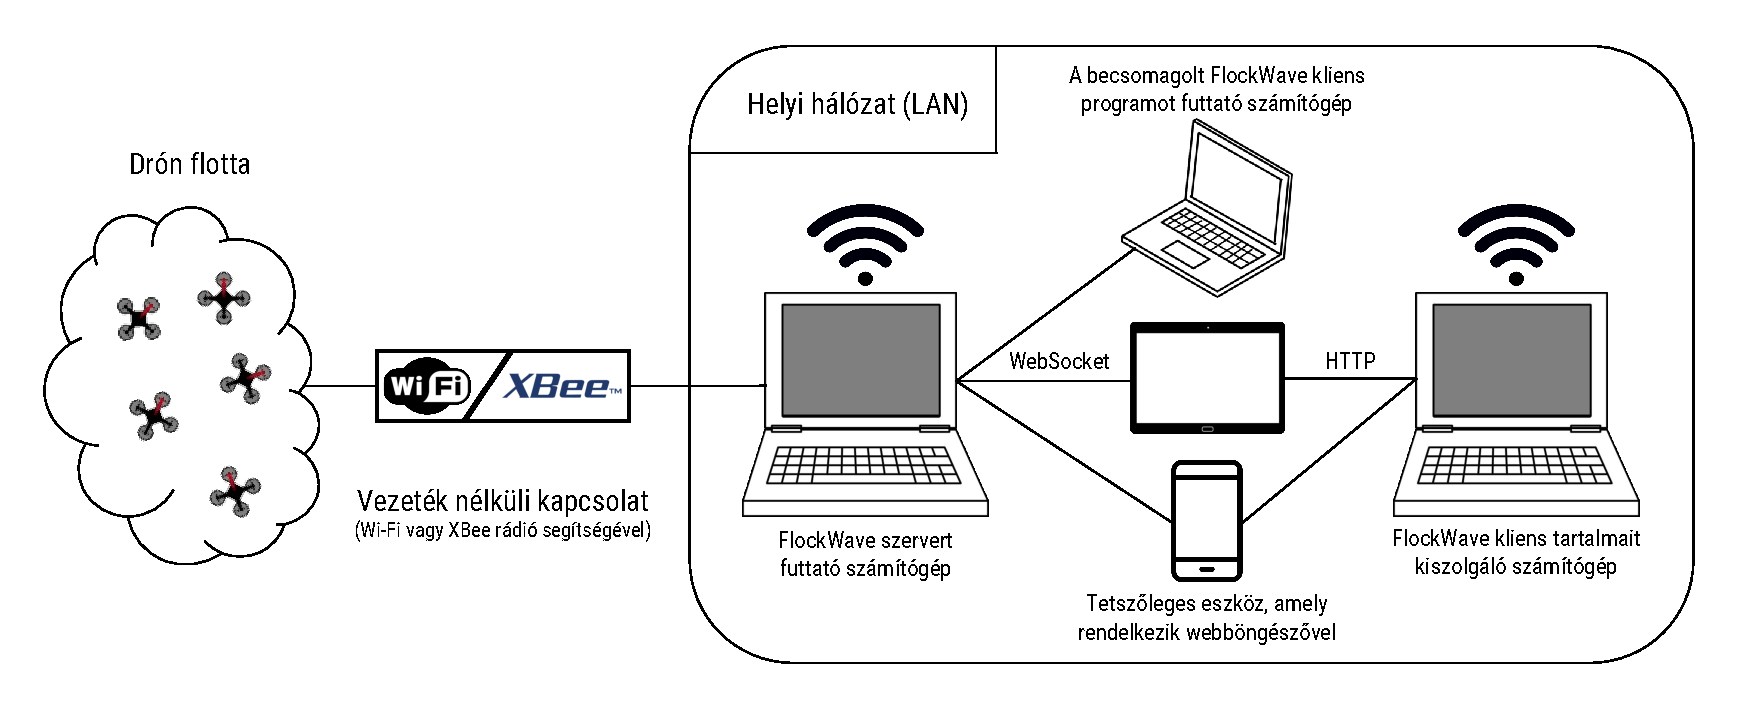
\includegraphics[width=\textwidth]{operational_structure_2.pdf}
  \caption{A rendszer felépítése}
\end{figure}

\textit{Megjegyzés: Természetesen semmi sem zárja ki, hogy a FlockWave szerver
futtatását és a kliens tartalmának kiszolgálását ugyanaz a számítógép végezze.}
